\section{Introduction}
	This paper will explore continuous integration and continuous deployment (CI/CD) using a very basic sample NodeJS app designed with ReactJS. The practical element of this paper will implement CI/CD using a Jenkins server and AWS EC2 Container Service. The app will be deployed by a Jenkins build server  through the following workflow:
	
	\begin{enumerate}
		\item Developer performs a \textit{git push} of the apps source code to GitHub;
		\item GitHub, detecting the \textit{push}, uses a \textbf{webhook} to a Jenkins Server to trigger a \textbf{Jenkins job};
		\item A Jenkins job starts and completes the following build steps:
		\begin{enumerate}
			\item Pulls the source code of the app, the including a \textbf{Dockerfile}, and builds an image;
			\item Pushes the image to a \textbf{Docker Hub registry};
			\item Creates a new \textbf{task definition} on ECS specifying the new image as the source Docker image;
			\item Updates an ECS \textbf{Service} to launch the new task definition on an \textbf{ECS instance}.
		\end{enumerate}
		\item The ECS service starts the desired number of task definitions in place of older version(s);
		\item The task definition(s) pull the image from Docker Hub and run it in a container on the ECS instance.
	\end{enumerate}
	Terms highlighted above will be explored in the practical report.
	
	\begin{figure}[H]
		\caption{Workflow Overview}
		\centering
		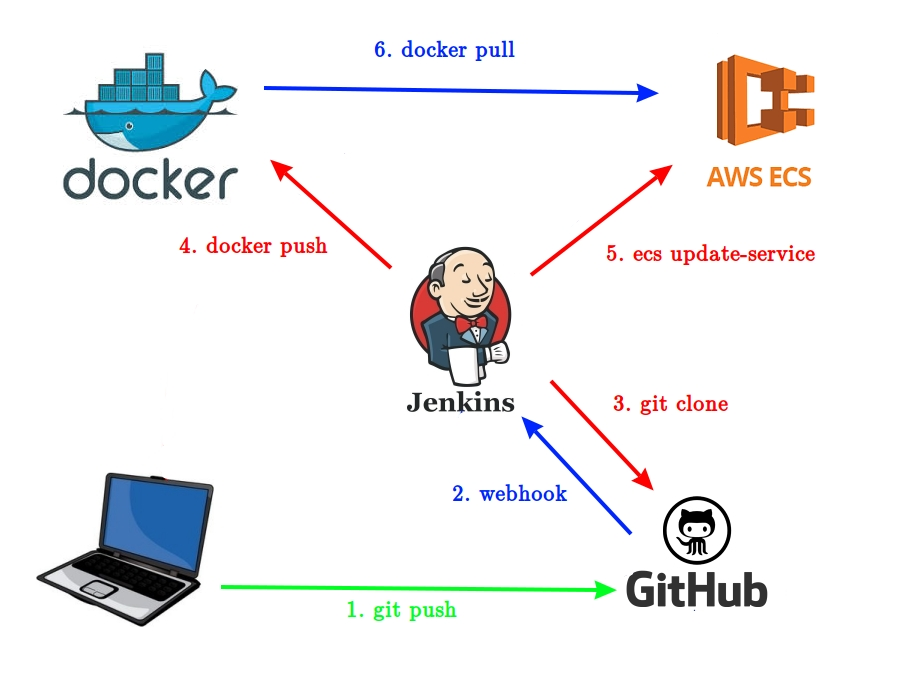
\includegraphics[width=0.8\textwidth,keepaspectratio]{overview}
		\label{fig:overview}
	\end{figure}

	\subsection{Objectives}
	Based on the above work to be completed and the services which will be utilised, the paper has four main objectives:
	\begin{itemize}
		\item Implement a CI/CD pipeline for a simple web app.
		\item Examine the use of a number of Jenkins plugins to allow the execution of various build steps within a Jenkins job.
		\item Explore AWS'  EC2 Container Server
		\item Examine the use of AWS' IAM service as a method of securely allowing users and services to perform task on AWS.
	\end{itemize}
	
	\subsection{Background}
	CI/CD is interchangeably referred to as Continuous Integration/Continuous Deployment and Continuous Integration/Continuous Delivery. In order to implement a CI/CD workflow as part of this paper it is worth first understanding what each of these terms means. This will provide a better understanding of the objective of this paper and indication as to whether continuous deployment or continuous delivery will be implemented.
	
	\subsubsection{Continuous Integration} CI is the easiest of the terms to define. It is the practice of continually preparing a product for release. This takes the form of developers continually committing their work to the source code as soon as any body of work has been completed. Commits to source code usually undergo some form of testing and building each time they are made. This means that code is constantly committed, tested and built at each iteration of development instead of when it comes to release time \citep{pittet}.
	
	The CI aspect of this project refers to the image build. Every time a commit is made to GitHub, the source code will be cloned by Jenkins and a Docker image built. As this is just a very basic sample web app there is no testing in place. However, testing before building is generally a main aspect on continuous integration.
	
	\subsubsection{Continuous Delivery} Continuous delivery is a step further than continuous integration. It refers to the act of continuously pushing the built code to a server. Thus, each time a commit is made and the code is tested and built (CI) it is then deployed to development server. Deploying the code to a production server must then be manually triggered if it is decided it is ready for release \citep{ellingwood}. 
	
	The continuous delivery element of this project refers to deploying the app to ECS where it can then be viewed by a web browser.
	
	\subsubsection{Continuous Deployment} Just as continuous delivery is a step beyond to continuous integration, continuous deployment is the next step. It removes the manual trigger to deploy to production servers. Therefore, code is constantly deployed to production at each commit, possibly many times a day \citep{ramos}.
	
	Although it may seem at first that this project is deploying straight to production, it will be observed later that this is not the case. The Dockerfile which defines how the image is built runs the Node app in development mode. This is not suitable for an app in production and therefore it cannot be said that this project implements continuous deployment.